Flash loans does not enable anything new it simply allows everyone to be able to trade with large amounts of capital (in one transaction), if you did indeed posses a vast amount of wealth (if you are a whale) then flash loans are not really of interest to you, you can already do the things it allows. With that in mind however, lets look at use cases for flash loans where most of them are interesting because everyone can now do them, not just a select few with a lot of capital. The following here is use-cases in which we can see the average trader participating in due to the possiblity presented by flash loans \cite{attack}.

\begin{wrapfigure}{r}{5.5cm}
  \centering
  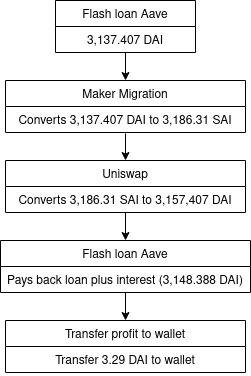
\includegraphics[width=.2\textwidth]{assests/Flash-loans-18-jan}
  \caption{A simplified figure showing the first arbitrage using flash loans.}
  \label{fig:firstArb}
\end{wrapfigure}
\paragraph{Arbitrage} An asset' value is determined through supply and demand, so if there is a larger supply of the asset than there is demand the price will go down and if the supply goes down (while the demand stays the same) the price goes up. This is reflected in the different DEX's, however they do enot instantly synchronize, so if one DEX trades an asset for a lower price than another, then there is an \textit{arbitrage} opportunity. Arbitrage is the process of making profit off of these prices difference. The prices differences will usually be small so in order to make a significant amount of money you will need a great deal of capital and this is where flash loans comes in. Flash loans guarentees that the loans is paid back at the end of the transaction, and arbitrage guarentees profit (if the trades back and forth in the exchanges is instantaneous) therefore you could consider arbitrage through flash loans risk-free, with the caveats that you do not count the vulnerabilities of smart contracts and you do not consider gas-fees a risk.

The first arbitrage, using flash loans, was reported by Camilla Russo on twitter\footnote{Camilla Russo twitter post \url{https://twitter.com/CamiRusso/status/1218640871048056832}}. We have illustrated a walkthrough of the arbitrage in figure \ref{fig:firstArb}, where we can see that the arbitrage opportunity lies in the exchange rate of Uniswap not matching the migration on MakerDAO.

\paragraph{Wash Trading} When tradeing it is important to have an eye on the trends of the market, what asset is frequently traded, how much of it, and why. Wash trading is the process of creating an artificial trend by buying and selling an asset thereby increasing the volume at which the asset is traded which will attract investors. This practice has been banned (in the USA) on the centralized markets since 1936. While we do not condone this practice it is undeniable a use-case for flash loans since with no significant captial can greatly increase the trade volume of an asset, and thereby manipulate the market.

\paragraph{Collateral Swapping} Lots of DeFi protocols allows you to put up collateral for loans, however there could be reasons for you wanting to change that collateral for example if your collateral is in ETH and the value of ETH declines, then you might want to swap it for DAI but you might have taken out loans aganist this collateral, so you do not have the capital to pay out your collateralized position and take out a new one in a different asset. With flash loans this becomes easy, you would loan the amount you need to pay out you position, swap that capital to the asset you want as the new collateral, take out a new collateralized position, and finally pay back the loan.